% Autor: Alfredo Sánchez Alberca (email:asalber@ceu.es)

\chapter{Formatting data}

Content of cells can be formatted in many ways: changing the data type, the font family, the alignment, the color, the
border, etc. Most formatting options are grouped in the \emph{Format Cells} dialog. To show this dialog click the bottom
right corner of the Font panel in the ribbon's Home tab.

\section{Data types}\hypertarget{data-types}{}\label{data-types}

Excel manages several data types. The most common are numbers, dates and times, and text. All available data types are
in the \texttt{Number tab} of the Format Cells dialog (see figure~\ref{img-number_dialog}).

\begin{figure}[htbp]
\begin{center}
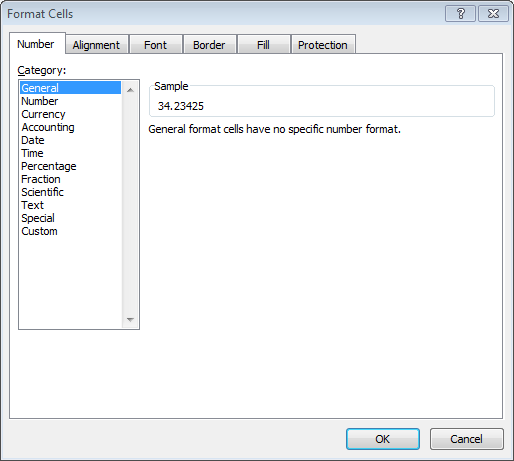
\includegraphics[scale=0.7]{../img/number_dialog.png}
\end{center}
\caption{Number dialog.}
\label{img-number_dialog}
\end{figure}

\subsection{Formatting numbers}\hypertarget{formatting-numbers}{}\label{formatting-numbers}

By default cells with numeric content are of type \emph{Number}, but there are other numeric types like \emph{Currency}
and \emph{Accounting}. Number is used for general display of numbers, while Currency and Accounting are used for
monetary values. In all cases you can specify the number of decimal places. For monetary values you can also specify the
symbol for the currency (\euro\ by default).

\textbf{Example}. The table in this \href{http://aprendeconalf.es/office/excel/manual/img/example_number_format.gif}{animation} shows the price of fruits during several months and the average price. The animation shows how to change the format of prices to currency type with 3 decimal places.

\subsection{Formatting dates and times}\hypertarget{formatting-dates-and-times}{}\label{formatting-dates-and-times}

By default cells with content following the pattern \texttt{day/month/year} are of type \emph{Date}, but there are a lot of ways of formatting dates, like for example, \texttt{year-month-day} or \texttt{day-month\_name-year} etc.

\textbf{Example}. The table in this \href{http://aprendeconalf.es/office/excel/manual/img/example_date_format.gif}{animation} shows the price of fruits during several months and the average price. The animation shows how to change the format of dates following the pattern Month-Year, with the three first letters of months and the two last digits of years.

By default cells with content following the pattern \texttt{hours:minutes:seconds} are of type \emph{Time}, but there are a several ways of formatting times.

\subsection{Formatting text}\hypertarget{formatting-text}{}\label{formatting-text}

By default cells with non numeric content are of type \emph{Text}. It's possible to apply this type even to numbers, like for example phone numbers.

Text entered in a cell spreads to adjacent cells to the right if these cells have no content. To confine text to a certain width in the cell, select the cell and click the button \texttt{Wrap Text} in the Alignment section in the ribbon's Home tab.

\section{Align cell contents}\hypertarget{align-cell-contents}{}\label{align-cell-contents}

By default numbers are aligned to the right and text to the left, but it's possible to change the alignment of cell
contents in the \texttt{Alignment tab} of the Format Cells dialog (see figure~\ref{img-alignment_dialog}).

\begin{figure}[htbp]
\begin{center}
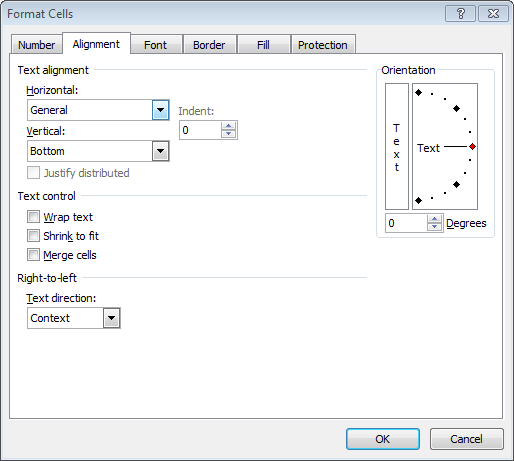
\includegraphics[scale=0.7]{../img/alignment_dialog.png}
\end{center}
\caption{Alignment dialog.}
\label{img-alignment_dialog}
\end{figure}

\subsection{Horizontal alignment}\hypertarget{horizontal-alignment}{}\label{horizontal-alignment}

To change the horizontal alignment select Left, Right, Center or Justify in the Horizontal drop down list of the
\texttt{Alignment tab}. You can also align the cell contents with the buttons of the Alignment panel in the Home tab of
the ribbon (see figure~\ref{img-button_horizontal_alignment}).

\begin{figure}[htbp]
\begin{center}
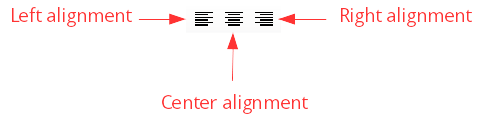
\includegraphics[scale=0.7]{../img/button_horizontal_alignment.png}
\end{center}
\caption{Horizontal alignment buttons.}
\label{img-button_horizontal_alignment}
\end{figure}

\textbf{Example}. The table in this \href{http://aprendeconalf.es/office/excel/manual/img/example_alignment.gif}{animation} shows the price of fruits during several months and the average price. The animation shows how to align the average prices centered.

\subsection{Vertical alignment}\hypertarget{vertical-alignment}{}\label{vertical-alignment}

To change the vertical alignment select Top, Bottom, Center or Justify in the Vertical drop down list of the
\texttt{Alignment tab}. You can also align the cell contents with the buttons of the Alignment panel in the Home tab of
the ribbon (see figure~\ref{img-button_vertical_alignment}).

\begin{figure}[htbp]
\begin{center}
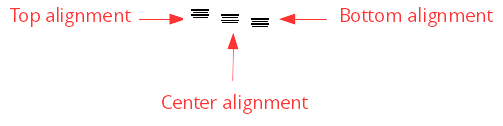
\includegraphics[scale=0.7]{../img/button_vertical_alignment.png}
\end{center}
\caption{Vertical alignment buttons.}
\label{img-button_vertical_alignment}
\end{figure}

\section{Font properties}\hypertarget{font-properties}{}\label{font-properties}

To format the font of cell contents select the font family, font style, font size and font color from the \texttt{Font
tab} of the Format Cells dialog (see figure~\ref{img-font_dialog}). You can also apply some effects like underline, superscript
and subscript.

\begin{figure}[htbp]
\begin{center}
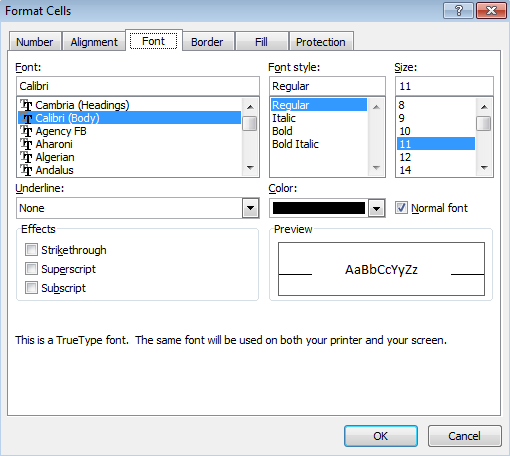
\includegraphics[scale=0.7]{../img/font_dialog.png}
\end{center}
\caption{Font dialog.}
\label{img-font_dialog}
\end{figure}

It's also possible to change the font family, style, size and color from the Font panel in the ribbon's Home tab, and also with the contextual toolbar that appears right-clicking the cell.

\textbf{Example}. The table in this
\href{http://aprendeconalf.es/office/excel/manual/img/example_font_family.gif}{animation} shows the price of fruits
during several months and the average price. The animation shows how to change the font family of all table to Arial,
size 10 pt. 

And this \href{http://aprendeconalf.es/office/excel/manual/img/example_font_colour.gif}{animation} also shows how
to change the font style of average prices to bold and the color of fruits names to blue.


\section{Borders and background}\hypertarget{borders-and-background}{}\label{borders-and-background}

To format the borders of cells select the line style and color, and click the borders where to apply that line in the
table of the \texttt{Borders tab} in the Format Cells dialog (see figure~\ref{img-border_dialog}).

\begin{figure}[htbp]
\begin{center}
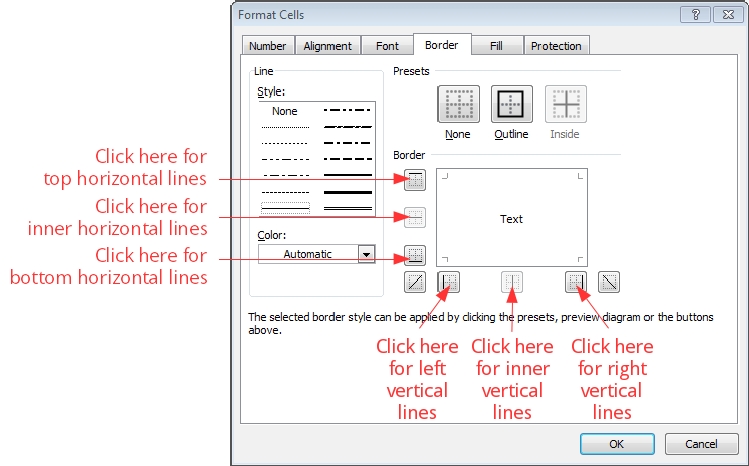
\includegraphics[scale=0.7]{../img/border_dialog.png}
\end{center}
\caption{Border dialog.}
\label{img-border_dialog}
\end{figure}

It's also possible to change the border of cells with the \texttt{Border button}
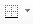
\includegraphics[scale=0.7]{../img/button_border.png} of the Font panel in the ribbon's Home tab, and also with the
contextual toolbar that appears right-clicking the cell.

\textbf{Example}. The table in this
\href{http://aprendeconalf.es/office/excel/manual/img/example_borders.gif}{animation} shows the price of fruits during several months and the average price. The animation shows how to put lines to some cell borders.

To format the background of cells select the background color and pattern style in the \texttt{Fill tab} of the Format
Cells dialog (see figure~\ref{img-fill_dialog}).

\begin{figure}[htbp]
\begin{center}
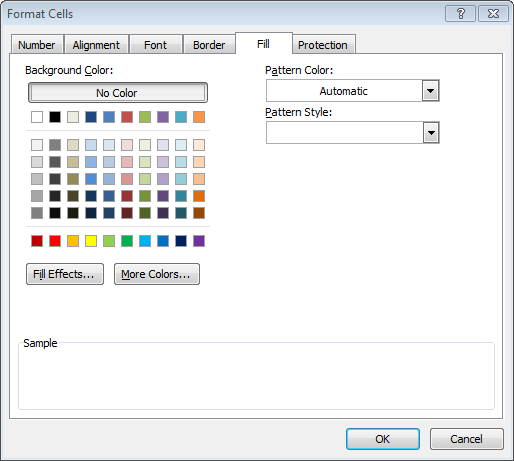
\includegraphics[scale=0.7]{../img/fill_dialog.png}
\end{center}
\caption{Fill dialog.}
\label{img-fill_dialog}
\end{figure}

It's also possible to change the background color of cells with the \texttt{Background colour} button 

\includegraphics[scale=0.7]{../img/button_background_colour.png} of the Font panel in the ribbon's Home tab, and
also with the contextual toolbar that appears right-clicking the cell.

\textbf{Example}. The table in this \href{http://aprendeconalf.es/office/excel/manual/img/example_background_colour.gif}{animation} shows the price of fruits during several months and the average price. The animation shows how set the background colour of some cells.

\section{Merge cells}\hypertarget{merge-cells}{}\label{merge-cells}

To merge several cells in one, select the range of cells and click the button \texttt{Merge \& Center} in the Alignment
section in the ribbon's Home tab. If there are more than one cell with content in the range, merging will keep the
content of the upper-left cell only. By default content of merged cells is centered.

\textbf{Example}. The table in this \href{http://aprendeconalf.es/office/excel/manual/img/example_merge_cells.gif}{animation} shows the price of fruits during several months and the average price. The animation shows how merge the cells of the first row and center the title.

\section{Copy and paste format}\hypertarget{copy-and-paste-format}{}\label{copy-and-paste-format}

To apply the format of a cell to others select the cell, click the \texttt{Format painter} button 

\includegraphics[scale=0.7]{../img/button_format_painter.png} to copy the cell format. Then then select the range of
cells to paste the that format.

\textbf{Example}. The table in this \href{http://aprendeconalf.es/office/excel/manual/img/example_format_painter.gif}{animation} shows the price of fruits during several months and the average price. The animation shows how to apply the same format of the fruit rows to a new row for pineapples.

\section{Conditional formatting}\hypertarget{conditional-formatting}{}\label{conditional-formatting}

Excel allows to apply a format to a cell depending on its value and according to some rules. To set a new rule click the
\texttt{Conditional Formatting} button and select \texttt{New Rule}. There are different types of rules:

\begin{itemize}
\item \textbf{Format all cells based on their value} Applies a format style based on the value of the cell. There are 4 types of styles:


\begin{itemize}
\item \emph{2-Color Scale} Applies a colour in a continuous scale ranging from one colour for the minimum value or percentage to other colour for the maximum value or percentage.

\textbf{Example}. The table in this \href{http://aprendeconalf.es/office/excel/manual/img/example_conditional_formatting_colour_scale.gif}{animation} shows the price of fruits during several months and the average price. The animation shows how to apply to prices a colour background in a continuous scale from green (the minimum price) to red (the maximum price).
\item \emph{3-Color Scale} The same than 2-Color Scale but with a third intermediate colour in the scale.
\item \emph{Data bar} Plots an horizontal bar in each cell with a length proportional to the value of the cell.

\textbf{Example}. The table in this \href{http://aprendeconalf.es/office/excel/manual/img/example_conditional_formatting_data_bar.gif}{animation} shows the price of fruits during several months and the average price. The animation shows how to apply to prices a data bar format.
\item \emph{Icon Sets} Divide the distribution of selected cell values in several parts according to intervals or percentiles, assign an different icon to each part, and plot the corresponding icon in each cell.

\textbf{Example}. The table in this \href{http://aprendeconalf.es/office/excel/manual/img/example_conditional_formatting_icon_set.gif}{animation} shows the price of fruits during several months and the average price. The animation shows how to apply to prices an icon set format. The icon set has three icons: red is applied to values under the 33 percentile, yellow is applied to values between 33 and 67 percentiles, and green is applied to values over 67 percentile.
\end{itemize}
\item \textbf{Format only cells that contain} Applies a format to the cell if satisfies a logical condition.
\end{itemize}

\textbf{Example}. The table in this \href{http://aprendeconalf.es/office/excel/manual/img/example_conditional_formatting_logical_condition.gif}{animation} shows the price of fruits during several months and the average price. The animation shows how to apply to prices higher than 2 € a red colour.

\begin{itemize}
\item \textbf{Format only top or bottom ranked values} Applies a format to a number or percentage of top or bottom values.
\end{itemize}

\textbf{Example}. The table in this \href{http://aprendeconalf.es/office/excel/manual/img/example_conditional_formatting_top_values.gif}{animation} shows the price of fruits during several months and the average price. The animation shows how to apply to the three top higher prices a red colour.

\begin{itemize}
\item \textbf{Format only values that are above or below average} Applies a format to cells with values above or below the average of selected cells.
\end{itemize}

\textbf{Example}. The table in this \href{http://aprendeconalf.es/office/excel/manual/img/example_conditional_formatting_average.gif}{animation} shows the price of fruits during several months and the average price. The animation shows how to apply a red colour to prices above the average and a green colour to prices below the average.

\section{Predefined styles}\hypertarget{predefined-styles}{}\label{predefined-styles}

Excel has a lot of predefined styles for formatting cells and tables. To apply a predefined cell style click
\texttt{Cell Styles} button and select the desired style. It's possible to define new cell styles. For that select the
cell with the format to define as a style, click \texttt{Cell Styles} button and select \texttt{New Cell Style}
option. In the dialog that appears just give a name to the new style, press OK, and the new cell style will appear in
the cell styles menu.

To apply a predefined table style click \texttt{Format as Table} button and select the desired style. It's also possible
to define new table styles. For that click \texttt{Format as Table} button and select \texttt{New Table Style} option.
In the dialog that appears just give a name to the new style, define the table format (font, borders and fill), press OK,
and the new table style will appear in the table styles menu.

